\section{Konventionen}
Bereits Rechnungen in der "`gewöhnlichen"' Relativitätstheorie haben die Tendenz
unübersichtlich zu werden, das Einführen zusätzlicher Dimensionen hilft dabei
natürlich kaum.
Es ist deshalb an dieser Stelle nützlich einige Konventionen festzulegen. Im
Folgenden bezeichnet $n$ die Anzahl der Zusatzdimensionen.\footnote{Im Weiteren
meist $n=1$}

Die Metrik soll stets die Signatur $(1,3)$, bzw. $(1,3+n)$, insbesondere sind
die Zusatzdimensionen. Die meisten Rechnungen werden in lokalen Koordinaten
durchgeführt.
Wir beginnen die Indizierung bei 0, wobei die 0. Komponente mit der Zeit identifiziert wird.
Griechische Indices laufen über ersten vier Raum-Zeit Koordinaten
$\mu=0,\ldots,3\,$, lateinische über alle inklusive der
Zusatzkomponenten \footnote{Verwirrung bezüglich der gängigen Konvention
mit lateinischen Indices die Raumkomponenten zu benennen sollte dabei nicht
aufkommen.}, $i=0,\ldots,3+n\,$. Weiter verwenden wir die Einsteinsche
Summenkonvention, d.h. über paare von Indizes wird implizit summiert.

Im Zusammenhang mit Zusatzdimensionen tauchen Größen auf, die sowohl ein 4, als
auch ein $4+n$ dimensionales Pendant besitzen. Um diese von einander zu
unterscheiden, kennzeichnen wir die $4+n$ dimensionale Version mit einem
Zirkumflex.
Beispielsweise bezeichnen wir den $4+n$ dimensionalen Ricci-Tensor mit
$\tensor{\hat{R}}{_i_j}$. Mit $g$ bezeichnen wir die Determinante der Metrik.
\subsection*{Geometrisierte Einheiten}
Wir verwenden geometrisierte Einheiten, d.h. Einheiten in denen
$8\pi G=c=1$. Es verbleibt nur noch eine Längendimension.
\chapter{Mathematische Grundlagen}
Die meisten KK-Theorien machen in der einen oder anderen Form Annahmen über
Symmetrien der Raumzeit-Mannigfaltigkeit. Dies ist nötig um die Komplexität der
auftretenden Ausdrücke zu reduzieren und nicht zuletzt auch dafür diese mit der
physikalischen Realität in Verbindung zu setzen, die zusätzlichen Dimensionen
müssen sich schon deshalb von den ersten vier unterscheiden, da sie nicht
(direkt) beobachtet werden können.
In diesem Kapitel werden wir die mathematischen Grundlage zur Formulierung von
Symmetrien in der Physik legen. Zunächst führen wir einige Begriffe der Differentialgeometrie
ein.
\section{Differentialgeometrie}
Eine Verallgemeinerung von des kartesischen Produkts $B\times F$ stellen
Faserbündel dar, die \emph{lokal} Produktstruktur besitzen. 
\begin{definition}[Faserbündel]
Seien $E,B,F$ topologische Räume, $\pi:E\to B$ eine stetige Surjektion.
Das Tupel $(E,B,\pi,F)$ heißt \emph{Faserbündel},
falls für jedes $x\in E$ eine offene Umgebung $U\subseteq B$ und ein
Homöomorphismus $\varphi:\pi^{-1}(U)\to U\times F$ existiert, sodass das folgende Diagramm kommutiert:
\begin{center}
\begin{tikzpicture}
\node[scale=1.3] at (0,0) {
\begin{tikzcd}
E \arrow{r}{\varphi} \arrow[swap]{d}{\pi} & U\times F
\arrow{dl}{\operatorname{proj}_1}\\
U & 
\end{tikzcd}
};
\end{tikzpicture}\,,
\end{center}
wobei $\operatorname{proj}_1:U\times F \to U$, die kanonische Projektion
bezeichnet. Die Menge aller $\{(U_x,\varphi_x)\}$ heißt \emph{lokale
Trivialisierung} des Bündels. Für $p\in B$ heißt $\pi^{-1}(\{p\})$
\emph{Faser} über $p$.  
Ein Faserbündel heißt \emph{glatt},
falls $E,B,F$ glatte Manigfaltigkeiten sind und $\pi$ sowie die alle $\varphi_x$
glatt sind.
\end{definition}
\begin{beispiel}[Triviales Bündel]
Seien $M,N$ glatte Mannigfaltigkeiten, dann ist $E=M\times N$ ein glattes
Faserbündel, eine lokale Trivialisierung
ist gegeben durch $\{(M,\id_{M\times N})\}$.
\end{beispiel}
Ein Beispiel für ein nicht triviales Bündel, ist die Kleinsche Flasche
(\autoref{fig:KleinFlasch}). 
\begin{figure}[hbtp!]
\centering
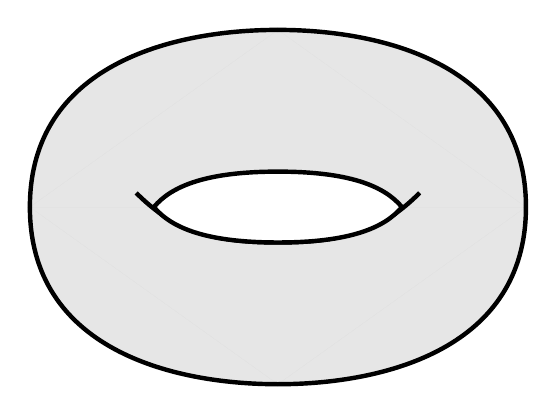
\begin{tikzpicture}[baseline,scale=0.9]
% \draw[dashed] (1.3,-1.33) [partial ellipse= 90:270:0.5cm and 1cm];
% \draw[dashed] (-1.3,-1.33) [partial ellipse=90:-90:0.5cm and 1cm];
%  \draw[thick, red,dashed] (-0,-1.5) [partial ellipse=270:90:0.4cm and 1cm];
%   \node[fill=white] at (0.7,-1.2) {$p$};
% \node at (0.4,-1.5){\textbullet};
%  \node at (1.8,-1.3){\textbullet};
% \node at (-1.8,-1.3){\textbullet};
\fill[fill=gray,fill opacity = 0.2]  (-3.5,0) -- (0, 2.5)  -- (3.5,0);
\fill[fill=gray,fill opacity = 0.2]  (-3.5,0) -- (0, -2.5)  -- (3.5,0);
\draw[fill=gray,fill opacity = 0.2,ultra thick] (-3.5,0) .. controls (-3.5,2)
and (-1.5,2.5) .. (0,2.5);
\draw[xscale=-1,fill=gray,fill opacity = 0.2,ultra thick] (-3.5,0) .. controls
(-3.5,2) and (-1.5,2.5) .. (0,2.5);
\draw[rotate=180,fill=gray,fill opacity = 0.2,ultra thick] (-3.5,0) .. controls
(-3.5,2) and (-1.5,2.5) .. (0,2.5);
\draw[yscale=-1,fill=gray,fill opacity = 0.2,ultra thick] (-3.5,0) .. controls
(-3.5,2) and (-1.5,2.5) .. (0,2.5);

\draw[,ultra thick] (-2,.2) .. controls (-1.5,-0.3) and (-1,-0.5) .. (0,-.5) ..
controls (1,-0.5) and (1.5,-0.3) .. (2,0.2);

\draw[fill=white,ultra thick] (-1.75,0) .. controls (-1.5,0.3) and (-1,0.5) ..
(0,.5) .. controls (1,0.5) and (1.5,0.3) .. (1.75,0);
\draw[fill=white,ultra
thick] (-1.75,0) .. controls (-1.5,-0.3) and (-1,-0.5) .. (0,-.5) .. controls (1,-0.5) and (1.5,-0.3) .. (1.75,0);
% \draw[thick, red] (-0,-1.5) [partial ellipse=90:-90:0.4cm and 1cm];
% \draw (1.3,-1.33) [partial ellipse=90:-90:0.5cm and 1.cm];

% \draw (-1.3,-1.33)  [partial ellipse=270:90:0.5cm and 1cm];

% \draw[gray] (-0,0) [partial ellipse=-180:0:3.5cm
% and 1.5cm]; %\draw[thick,  blue!80!black] (-0,0) [partial
% ellipse=-110:-70:3.5cm and 1.5cm];
\end{tikzpicture}
\quad
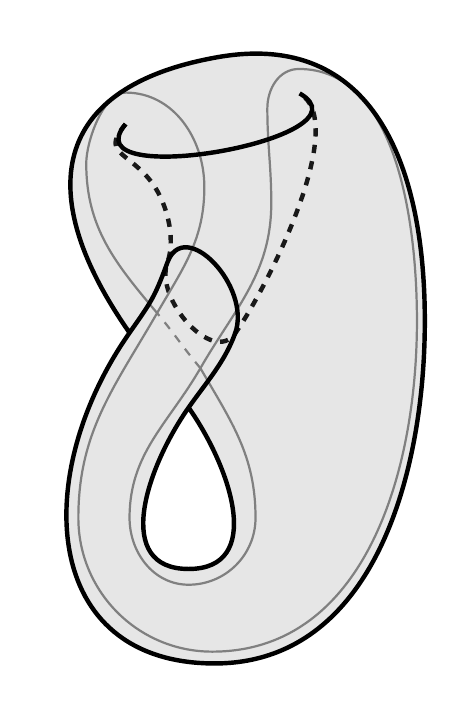
\begin{tikzpicture}[baseline]
\node (A) at (-1.45,0.35) {};
\node (B) at (-0.33,3.85){};
\node (C) at (-0.3683,-3.85) {};
\node (D) at (-0.97,1.24) {};
\node (E) at (-0.11,0.34) {};

\node (H) at (-0.7,-0.6){};
\node (I) at (-0.7,-2.65){};
\node (J) at (-0.7,-2.65){};
\node (K) at (2.3,0.5){};

\node (F) at (-1.5,3) {};
\node (G) at (0.71,3.39){};
\node (L) at (-1.2,2.3){};

\node (i1) at (-1.1,0.6) { };
\node (i2) at (-2,2.5)  { };
\node (i3) at (-1.5,3.4) { };
\node (i4) at (-0.5,2.2) { };
\node (i5) at (-2.1,-2) { };
\node (i6) at (-0.4,-3.7) { };
\node (i7) at (2.2,0.5) { };
\node (i8) at (0.7,3.7) { };
\node (i9) at (0.3,3.2) { };
\node (i10) at (0.35,2) { };
\node (i11) at (-0.55,-0.1) {};
\node (i12) at (-1.45,-2) { };
\node (i13) at (-0.7,-2.85) { };
\node (i14) at (0.15,-2) { };


\draw[dashed, ultra thick] (F.center)
to[out=230, in =130,looseness=1.6] (L.center)
to[out=180+130, in =180+250,looseness=0.8] (D.center)
to[out =250,in=235] (E.center)
to[out =235+180,in=180-210,looseness=0.6] (G.center);

\draw[fill=gray,draw=none,fill opacity=0.2]
(A.center)
to[out= -235,in=190,looseness=1.5] (B.center)
to[out=10, in = 90,looseness=1.2] (K.center)
to[out=-90, in = 0,looseness=1.] (C.center)
to[out=180, in = 235,looseness=1.3] (A.center)
to[out=235+180, in = 250,looseness=1.2] (D.center)
to[out=250+180, in = 250+180,looseness=1.3] (E.center)
to[out=250, in = 235+180,looseness=0.9] (H.center)
to[out=235, in = 180,looseness=1.2] (I.center)
to[out=0, in = 180-235,looseness=1.2] (H.center)
--cycle
;

\draw[thick,gray] (i1.center)
to[out= 130, in = 90+180] (i2.center)
to[out =90,in=180,looseness=0.7] (i3.center)
to[out=0,in=90] (i4.center)
to[out=180+90,in=180-120] (i1.center)
to[out=-120,in=90] (i5.center)
to[out=-90,in=180] (i6.center)
to[out=0,in=-90] (i7.center)
to[out=90,in=0,looseness=0.9] (i8.center)
to[out=180,in=90] (i9.center)
to[out=-90,in=90] (i10.center)
to[out=-90,in=180-120] (i11.center)
to[out=-120,in=90] (i12.center)
to[out=-90,in=180] (i13.center)
to[out=0,in=-90] (i14.center)
to[out=90,in=180+120] (i11.center);
to[out=130,in=180+130,dashed] (i1.center);

\draw[dashed,thick,gray] (i11.center) to[out=130,in=180+130] (i1.center);
\draw[ultra thick](A.center)
to[out= -235,in=190,looseness=1.5] (B.center)
to[out=10, in = 90,looseness=1.2] (K.center)
to[out=-90, in = 0,looseness=1.] (C.center)
to[out=180, in = 235,looseness=1.3] (A.center)
to[out=235+180, in = 250,looseness=1.2] (D.center)
to[out=250+180, in = 250+180,looseness=1.3] (E.center)
to[out=250, in = 235+180,looseness=0.9] (H.center)
to[out=235, in = 180,looseness=1.2] (I.center)
to[out=0, in = 180-235,looseness=1.2] (H.center);

\draw[ultra thick] (F.center) to[out=230, in =180-210,looseness=1.3] (G.center);
\end{tikzpicture}
\caption{Torrus und Kleinsche Flasche sind Beispiele
für $\Sphere^1$-Faserbündel über $\Sphere^1$.}
\label{fig:KleinFlasch}
\end{figure}
\subsection{Äußeres Kalkül}
Äußere Ableitung, Hodge Dual, Wedge Produkt
\section{Symmetrien}
Wir beginnen mit einem einfachen Beispiel für eine Symmetrie, dass uns auch im
Folgenden als Anschauungsobjekt dienen wird.
\begin{beispiel}[Symmetrien eines Zylinders]
Wir betrachten einen Zylinder
\begin{equation}
Z=\Reals\times\Sphere^1=\left\{(x,y,z)\in\Reals^3\,\Big|\,x^2+y^2=1\right\}\,,
\end{equation}
als Teilmenge des $\Reals^3$.
Offensichtlich besitzt dieser zwei Symmetrien. Zum Einen wird er durch
Drehung um die $z$-Achse in sich selbst überführt (Rotationsinvarianz), zum
Anderen können wir den Ursprung entlang der $z$-Achse beliebig wählen
(Translationsinvarianz).
\end{beispiel}
Eine formale Beschreibung solcher kontinuierlicher Symmetrien bieten 
Gruppen die zusätzlich eine differenzierbare Struktur besitzen.
\begin{definition}[Lie-Gruppe]
Sei $G$ eine glatte Mannigfaltigkeit, versehen mit einer Gruppenstruktur
$(G,*)$.
Sind die Multiplikation $m:(g,h)\mapsto g* h$ und Inversion $i:g\mapsto g^{-1}$
glatt, so heißt $G$ \emph{Lie-Gruppe}.
\end{definition}
%TODO Lie Algebren
\begin{bemerkung}
Der Zylinder $Z$ besitzt offensichtlich auch eine Spiegelsymmetrie bezüglich der
Koordinatenachsen. Dabei
handelt es sich aber um eine diskrete Symmetrien, welche sich nicht durch Lie-Gruppen beschreiben lassen.
\end{bemerkung}
\begin{beispiel}[$\SpOr(n)$]% TODO
\end{beispiel}
In unserem Fall ist die Lie-Gruppe die die Operationen beschreibt die Gruppe der
Drehungen um die $z$-Achse. Diese wird mit $\SpOr(2)$ bezeichnet, eine
Darstellung ergibt sich beispielsweise durch Matrizen der Form
\begin{equation}
R(\alpha)=
\begin{pmatrix}
\cos\alpha&\sin\alpha&0\\
-\sin\alpha&\cos\alpha&0\\
0&0&1
\end{pmatrix}
\end{equation}
%TODO zusammenhang SO(2) und R/Z
Das diese Gruppe eine differenzierbare Struktur besitzt ist klar da die
Komponenten der Matrizen differenzierbar sind.
Gruppen können auf Mengen operieren.  
Allgemeiner wollen wir nun definieren wie die Wirkung einer Gruppe auf einer
Menge zu verstehen ist. Eine sinnvolle Operation einer Gruppe sollte dabei mit
den Gruppenoperationen kompatibel sein.
\begin{definition}[Gruppenwirkung]
Sei $G$ eine Gruppe, $X$ eine Menge. Eine Abbildung
\begin{equation}
\Phi:G\times X\to X\,,\quad (g,x)\mapsto\Phi_g(x)
\end{equation}
heißt \emph{Gruppenwirkung} von $G$ auf $X$, falls die folgende Eigenschaften
erfüllt sind
\begin{enumerate}
  \item \emph{Identität}: für das neutrale Element $e\in G$ gilt
  $\displaystyle\Phi_e=\id_X$
  \item \emph{Verträglichkeit}: $\displaystyle\Phi_{gh}=\Phi_g\circ\Phi_h$
\end{enumerate}
$X$ heißt dann auch $G$-Menge.
\end{definition}
Statt $\Phi_g(x)$ schreiben wir kurz $g\gmal x$.
Ist die Gruppe $G$ eine Lie-Gruppe, $X=M$ eine Mannigfaltigkeit und $\Phi_g$
glatt, so spricht man von einer \emph{Lie-Gruppenwirkung}. $M$ heißt dann
auch $G$-Mannigfaltigkeit.
\begin{definition}
Sei $X$ eine $G$-Menge. Die Wirkung von $G$ heißt:
\begin{enumerate}
  \item \emph{eigentlich}, falls unter der Abbildung $\Gamma:
  G\times X\to X\times X\,,(g,x)\mapsto (g \gmal x,x)$, Urbilder kompakter
  Mengen kompakt sind
  \item \emph{(Fixpunkt-)frei}, falls nur die Identität Fixpunkte besitzt, d.h.
  aus $g\gmal x=x$, folgt $g=e$.
\end{enumerate}
\end{definition}
\begin{beispiel}[Wirkung von $\Reals/\Integers$ auf $Z$]
Sei $G=(\Reals/\Integers,+)$, $Z$ wie oben. Eine Wirkung von $G$ auf $Z$ ist
erklärt durch
\begin{equation}
t.p= \begin{pmatrix}
\cos\left( 2\pi t\right)&\sin\left( 2\pi t\right)&0\\
-\sin\left( 2\pi t\right)&\cos\left( 2\pi t\right)&0\\
0&0&1
\end{pmatrix}p\,,\quad p\in Z\subseteq \Reals^3
\end{equation}
Wie man sich leicht klar macht ist die Wirkung glatt, frei und eigentlich.
\end{beispiel}
\begin{figure}[!htbp]
\centering
\begin{tikzpicture}
\draw[-latex] (2,1)-- (-2,-1)  ;
\draw[-latex]  (-2,1)--(2,-1)  ;
\draw[fill=white,draw=none] (-1,4) -- (-1,0) arc (180:360:1cm and 0.5cm) -- (1,4) arc (-180:0:-1cm and 0.5cm) ;
\draw[fill=white,draw=none] (0,4) ellipse (1cm and 0.5cm);
\draw[-,thick, dashed] (0,-0.5) -- (0,4) ;
\draw[dashed] (2,1)-- (-2,-1)  ;
\draw[dashed]  (-2,1)--(2,-1)  ;
\draw[-,thick] (0,-1) -- (0,-0.5) ;
\node at (0,0) {\tiny\textbullet};
\node at (0,4) {\tiny\textbullet};
\draw[densely dashed] (-1,2) arc (180:0:1cm and 0.5cm);
\draw[fill=gray,fill opacity = 0.1,draw=none] (0,4) ellipse (1cm and 0.5cm);
\draw[fill=gray,fill opacity = 0.2] (-1,4) -- (-1,0) arc (180:360:1cm and 0.5cm) -- (1,4) arc (-180:0:-1cm and 0.5cm) ;
\draw[densely dashed] (-1,0) arc (180:0:1cm and 0.5cm);
\draw(-1,4) arc (180:0:1cm and 0.5cm);
\draw[densely dashed]  (-1,2) arc (-180:0:1cm and 0.5cm);
\draw[thick, red, -latex] (0,2) [partial ellipse=-60:-140:1cm and 0.5cm];
\node at (2.2,4) {$Z=\mathbb{R}\times\mathbb{S}^1$};
\node at (2+0.3,-1-0.2) {$y$};
\node at (-2+0.3,-1-0.2) {$x$};
\node at (0.3,5) {$z$};
\node at (0.5,1.25) {$p$};
\draw[-latex,thick] (0,4) -- (0,5) ;
\node at (0.51,1.57){\textbullet};
\end{tikzpicture}
\caption{Wirkung von $\Reals/\Integers$ auf dem Zylinder $Z$.}
\end{figure}
\section{Orbiträume}
Die Wirkung einer Gruppe definiert in natürlicher
Weise Äquivalenzklassen auf einer Mannigfaltigkeit, welche gerade diejenigen
Elemente enthalten, die sich durch $G$-Wirkung ineinander überführt werden.
Eine solche Äquivalenzklasse nennen wir Bahn oder Orbit.
\begin{definition}[Orbit]
Sei $X$ eine $G$-Menge, $x\in X$, dann heißt die Menge
\begin{equation}
G \gmal x=\{g \gmal x\,|\,g\in G\}
\end{equation}
\emph{Orbit} von $x$. Als \emph{Orbitraum} bezeichnen wir die Menge aller Orbits
\begin{equation}
M/G=\{[x]=G.x\,|\,x\in M\}\,,
\end{equation}
versehen mit der Quotiententopologie, der gröbsten Topologie für die die
kanonische Projektion $x\mapsto [x]$ stetig ist.
\end{definition}
\begin{beispiel}[Orbits von $\Reals/\Integers$ auf $Z$]
Wenn wir wieder das Beispiel $G=(\Reals/\Integers,+)$, $M=Z$ heranziehen, so
sind die Orbits gegeben durch
\begin{equation}
G.(0,0,z)=\left\{(\sin (2\pi t),\sin (2\pi t),z)\,,t \in
[0,1)\right\}\cong\Sphere^1\,.
\end{equation}
Der Orbitraum $M/G$ selbst ist offensichtlich diffeomorph zu $\Reals$. Der
Zylinder lässt sich also lokal als Produkt von Orbitraum und Orbit darstellen.
\end{beispiel}
\begin{figure}[!htbp]
\centering
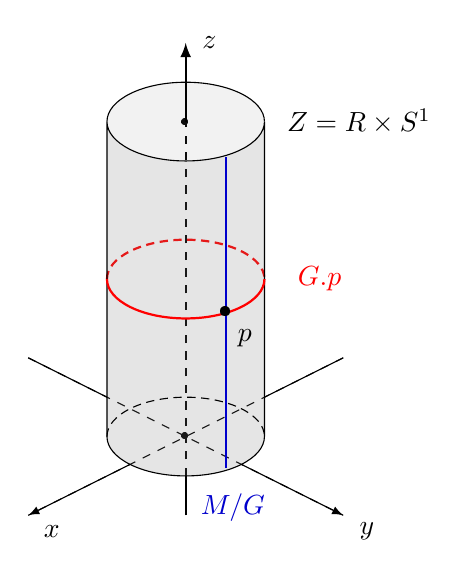
\begin{tikzpicture}
\draw[-latex] (2,1)-- (-2,-1)  ;
\draw[-latex]  (-2,1)--(2,-1)  ;

\draw[fill=white,draw=none] (-1,4) -- (-1,0) arc (180:360:1cm and 0.5cm) -- (1,4) arc (-180:0:-1cm and 0.5cm) ;
\draw[fill=white,draw=none] (0,4) ellipse (1cm and 0.5cm);
\draw[-,thick, dashed] (0,-0.5) -- (0,4) ;
\draw[dashed] (2,1)-- (-2,-1)  ;
\draw[dashed]  (-2,1)--(2,-1)  ;
\draw[-,thick] (0,-1) -- (0,-0.5) ;
\node at (0,0) {\tiny\textbullet};
\node at (0,4) {\tiny\textbullet};
\draw[densely dashed,red,thick] (-1,2) arc (180:0:1cm and 0.5cm);
\draw[fill=gray,fill opacity = 0.1,draw=none] (0,4) ellipse (1cm and 0.5cm);
\draw[fill=gray,fill opacity = 0.2] (-1,4) -- (-1,0) arc (180:360:1cm and 0.5cm) -- (1,4) arc (-180:0:-1cm and 0.5cm) ;
\draw[densely dashed] (-1,0) arc (180:0:1cm and 0.5cm);
\draw(-1,4) arc (180:0:1cm and 0.5cm);
\draw[red,thick]  (-1,2) arc (-180:0:1cm and 0.5cm);
\draw[thick, blue!80!black] (0.51,-0.4)-- (0.51,3.55);
\node at (2.2,4) {$Z=\mathbb{R}\times\mathbb{S}^1$};
\node[red] at (1.7,2) {$G.p$};
\node[ blue!80!black] at (0.6,-0.9) {$M/G$};
\node at (2+0.3,-1-0.2) {$y$};
\node at (-2+0.3,-1-0.2) {$x$};
\node at (0.3,5) {$z$};
\node at (0.75,1.25) {$p$};
\draw[-latex,thick] (0,4) -- (0,5) ;
\node at (0.51,1.57){\textbullet};
;\end{tikzpicture}
\caption{Orbits der Wirkung der Gruppe $\Reals/\Integers$ auf $Z$.}
\end{figure}

Interessant sind insbesondere Fälle, in denen der Orbitraum selbst wieder eine
Mannigfaltigkeit darstellt. Dies muss allerdings im allgemeinen nicht der Fall
sein, wie das folgende Beispiel zeigt.
\begin{beispiel}[Ein nicht Hausdorffscher
Quotient \cite{abraham1978foundations}] Sei $G=(\Reals,+)$, $M=\Reals$ und $G$ wirke auf
$M$ durch $t \gmal x=e^tx$.

Der Quotient $M/G$ enthält die drei Äquivalenzklassen $[-1],[0],[1]$, da die
Abbildung das Vorzeichen nicht ändert.
Die Quotiententopologie $\tau$ lässt sich explizit angeben:
\begin{equation}
\tau =\big\{\emptyset,\{[-1]\},\{[1]\},\{[-1],[1]\},M/G\big\}\,.
\end{equation}
Offensichtlich ist die einzige Menge, die $[0]$ enthält $M/G$. Die Elemente
$[0],[1]$ lassen sich damit nicht durch offene Mengen trennen, d.h. $(M/G,\tau)$
ist nicht Hausdorff.
\begin{figure}[!htbp]
\centering
\begin{tikzpicture}
\draw [dashed](-3,0)--(-2,0);
\draw [dashed](3,0)--(2,0);
\draw (-2,0)--(-0.3,0);
\draw (2,0)--(0.3,0);
\node at (-1,-2){\textbullet};
\node at (0,-2){\textbullet};
\node at (1,-2){\textbullet};
\node at (4,0){$M=\mathbb{R}$};
\node at (4,-2){$M/G$};
%\draw[<-] (-1,-3)--(-0.8,0);
%\draw (-1,-3)--(-2.5,-2.5);
%\draw (1,-3)--(0,0) --(2,0) --cycle;
%\draw (0,-3)--(0,0)  --cycle;
\node at (0,0){\textbullet};
\node at (-1,-2.5){$[-1]$};
\node at (0,-2.5){$[0]$};
\node at (1,-2.5){$[1]$};
\node at (0,.5){$G.0$};
\node at (-1.3,.5){$G.(-1)$};
\node at (1.3,.5){$G.1$};
\node at (-0.3,0){$)$};
\node at (0.3,0){$($};
\end{tikzpicture}
\caption{Konstruktion eines nicht Hausdorffschen Quotienten.}
\end{figure}
\end{beispiel}
Tatsächlich scheitert die Konstruktion daran, dass die Wirkung nicht eigentlich
ist, beispielsweise ist das Urbild $\Gamma^{-1}\big([0,1]\times
\{1\}\big)=(-\infty,0]\times \{1\}$ nicht kompakt.
Vielmehr lässt sich zeigen dass der Quotient genau dann Hausdorff ist, wenn die
Gruppe eigentlich wirkt. %TODO REF

Wir geben nun eine Charakterisierung, die solche pathologische
Fälle ausschließt.
\begin{theorem}[Quotient Manifold Theorem \cite{lee2003smooth}]
Sei $G$ eine Lie-Gruppe, die glatt, frei und eigentlich auf einer glatten
Mannigfaltigkeit $M$ wirkt, dann ist der Orbitraum eine topologische
Mannigfaltigkeit der Dimension $\dim M/G=\dim M -\dim G$ und es existiert eine
eindeutige glatte Struktur sodass $\pi:M\to  M/G$ eine glatte Submersion ist.
\end{theorem}
\begin{korollar}
Sei $G$ eine Lie-Gruppe, die glatt, frei und eigentlich auf einer glatten
Mannigfaltigkeit $M$ wirkt. Dann ist $\pi:M\to M/G$ ein glattes Hauptfaserbündel,
mit Basis $M/G$ und typischer Faser $G$.
\end{korollar}
% Das Slice Theorem liefert, das falls $G$ kompakt und fixpunktfrei ist $M/G$ eine
% Manigfaltigkeitstruktur besitzt, bzw. sogar $M\to M/G$ ein $G$-Hauptfaserbündel
% ist.
% %http://math.stackexchange.com/questions/1315445/quotient-manifold-theorem-provides-a-fibrations
\section[Integration inv Fkt]{Integration auf Faserbündeln}
\begin{theorem}[Verallgemeinerter Fubini]\label{th:fubini}
Sei $M,N$, $m$ bzw. $n$-dimensionale, orientierbare Mannigfaltigkeiten, mit
$m\geq n$.
Sei $\varphi:M\to N$ glatt, $\omega$ eine $(m-n)$-Form auf $M$, sowie $\eta$
eine $n$-Form auf $N$. Sei $f:M\to \Reals$ Lebesgue integrabel, dann existiert 
für fast alle $p\in N$ eine messbare Funktion
\begin{equation}
F(p)=\int_{\varphi^{-1}(p)}f\omega\,,
\end{equation}
das \emph{Integral entlang der Faser}. Es gilt
\begin{equation}
\int_{M}f\omega\wedge\varphi^*\eta=\int_{N}F \eta\,.
\end{equation}
% Seien $M$, $N$ orientierbare Manigfaltigkeiten, $\pi$ die Projektion auf $M$
% bzw $N$, $\eta$, $\omega$ differentialformen auf $M$ bzw. $N$, $h:M\times N\to
% \Reals$ glatt, dann gilt
% \begin{equation}
% \int_{M\times N} h\pi_1^\star\eta\wedge\pi_2^\star\omega
% =\int_M g\eta\,,\quad g(p):=\int_N h(p,\cdot)\omega\,.
% \end{equation}
\end{theorem}
\begin{proof}
Siehe Sulantke und Wintgen
%Polynomial Convexity Edgar Lee Stout
\end{proof}
\begin{bemerkung}
Bei \autoref{th:fubini} handelt es sich um eine Verallgemeinerung, des aus der
Analysis bekannten Satzes von Fubini.
Sei $M=\Reals^m$, $N=\Reals^n$, und
\begin{align*}
\pi :M &\to N\\
(x_1,\dots,x_n,y_1,\dots,y_k) &\mapsto (x_1,\dots,x_n)\,.
\end{align*}
Wir definieren Differentialformen auf $N$ bzw. $M$ durch
$\omega=\dif{x}^1\wedge\cdots\wedge\dif{x}^n$ und
$\eta=\dif{x}^{n+1}\wedge\cdots\wedge\dif{x}^m$.
Nach\autoref{th:fubini}gilt
\begin{equation}
\begin{split}
\int_{\Reals^m} f\dif{}^m x &= \int_{\Reals^m}
f\dif{x}^1\wedge\cdots\wedge\dif{x}^n\wedge\dif{x}^{n+1}\wedge\cdots\wedge\dif{x}^m\\
&= \int_{\Reals^m}f\,\omega\wedge\pi^*\eta\\
&= \int_{\Reals^n}\left(\int_{\pi^{-1}(x)}f\,\omega\right)\eta\\
&= \int_{\Reals^n}\left(\int_{\{x\}\times\Reals^{(m-n)}}f\,\omega\right)\eta\,,
\end{split}
\end{equation}
was der bekannten Formel entspricht.
\end{bemerkung}
Ein interessantes Resultat ergibt sich wenn wir Funktionen betrachten, die
entlang der Fasern $\pi^{-1}(x)$ konstant sind.
\begin{definition}
Sei $X$ eine $G$-Menge, $Y$ eine Menge, $f:X\to Y$ mit
\begin{equation}
f(g\gmal p)=f(p)\,,\quad \forall g\in G\,,p\in E\,,
\end{equation}
dann heißt $f$ \emph{$G$-invariant}.
\end{definition}
Sei $G$ eine kompakte Lie-Gruppe dann gilt $\vol(G):=\int_G\dif h<\infty$
%TODO Beweis
.
Wir betrachten ein $G$-Hauptfaserbündel $\pi: E\to M$,
ausgestattet mit einer $G$-invarianten {(pseudo-)riemannschen} Metrik $g$.
Die Abbildung $f:E\to \Reals$ sei $G$-invariant und integrierbar. Dann gilt nach
\autoref{th:fubini}
\begin{equation}
\begin{split}
\int_E f\sqrt{g}\dif{}\hat{x}&=\int_{M}\int_{G}f\sqrt{g}\dif^{}h \dif x\\
&=\int_{M}f\sqrt{g}\int_{G}\dif^{}h \dif x\\
&=\vol(G)\int_{M}f\sqrt{g} \dif x\\
\end{split}
\end{equation}
Die Integration über den Totalraum $E$ kann also mit einer Integration über die
Basis $M$ identifiziert werden.
% TODO Maß über gruppe nöher untersuchen: s.126 Symmetrien
% und Gruppen in
% der Teilchenphysik
% Eine
% Tivialisierung einer offenen Menge $U\subset M=E/G$, ist ein Homoemorphismus
% \begin{equation}
% \Psi:\pi^{-1}(U)\to U\times G\,.
% \end{equation}
% Wir definieren eine Abbildung $\tilde{f}: M\to\mathrm{R}$
% \begin{equation}
% \tilde{f}\left(x\right):=\left(f\circ \Psi^{-1}\right)(x,e)\,.
% \end{equation}
% % Diese ist wohldefiniert, denn
% % \begin{equation}
% % \begin{split}
% % f\left(\Psi^{-1}(x,h)\right)&=f\left(\Psi^{-1}(x,h.e)\right)\\
% % &=f\left(h.\Psi^{-1}(x,e)\right)\\
% % &=f\left(\Psi^{-1}(x,e)\right)\,.
% % \end{split}
% % \end{equation}
% Damit gilt
% \begin{equation}
% \begin{split}
% \int_{\pi^{-1}(U)}f(x)\dif x&=
% \int_{\Psi\left(\pi^{-1}(U)\right)}\left[f\circ\Psi^{-1}\right](y,h)\dif y
% \dif h\\
% &=
% \int_{U\times G}\left[f\circ\Psi^{-1}\right](y,h)\dif y
% \dif h\\
% &=\int_G\int_{U}\tilde{f}\left(y\right)\dif y
% \dif h\\
% &=\vol (G)\int_{U}\tilde{f}\left(y\right)\dif y\,,\label{eq:Intprod}
% \end{split}
% \end{equation}
% Eine anschauliche Betrachtung $\tilde{f}$ als Mittelung der makroskopischen Funktion $f$ über die Zusatzdimension auffassen.
% Phsikalisch liegt ein solcher Fall vor, falls die Auflösung einer Messung zu
% gering ist um die kompakte Dimension zu beobachten. Bisher konnten kompakte
% Zusatzdimensionen nicht beobachtet werden, neue Erkentnisse bringt
% möglicherweise der 2015 gestarteten Lauf des Large Hadron Coliders am CERN. Die
% lokalen Trivialisierungen überdecken $M$, damit lassen sich auch Integrale auf dem gesammten Raum auf
% Integrale von der Form \eqref{eq:Intprod} zurückführen insbesondere gilt für die
% $G$-invariante Funktion $f\sqrt{g}$
% \begin{equation}
% \int_{E}f(x)\sqrt{g(x)}\dif x=\vol
% (G)\int_{M}\tilde{f}\left(y\right)\sqrt{\tilde{g}(y)}\dif y
% \end{equation}
% wobei $\tilde{g}(y)=\left[g\circ\Psi^{-1}\right](y,h)$. Im folgenden lassen wir
% die Tilden weg und identifizieren die Ausdrücke stillschweigend miteinander.
% Wir beenden dieses Kapitel mit einem Beispiel, der sogenannten
%\emph{ADM-decomposition}.
%\begin{beispiel}[ADM-decomposition]

%\end{beispiel}
\section{Variationsrechnung}
Variationsprinzipien stellen eine elegante Möglichkeit dar, physikalische
Theorien zu formulieren. Die Physik wird dabei durch einen Satz
von Parametern bzw. Funktionen beschrieben, die in gewisser Weise "`optimal"'
sind.
Wir orientieren uns in diesem Kapitel grob an den Ausführungen von \name{R.Wald}
\cite[s.454 ff]{wald2010general}.
Im folgenden bezeichne \emph{Feld} allgemein ein Tensorfeld, wobei wir den
Grad nicht angeben, sowie \emph{Feldkonfiguration} ein Tupel solcher
Feldern.

Wir wollen nun einen Formalismus entwickeln, der es erlaubt ein Funktional, nach
einer Funktion abzuleiten, um dadurch Extremalbedingungen in
Analogie zur klassischen Analysis zu formulieren.
Im Folgenden ist $X$ einen Banachraum, von Funktionen von einer Mannigfaltigkeit
$M$ in die reellen Zahlen, Typischerweise $X\subseteq C^\infty(M)$.
Weiter sei ein Funktional $I:X\to\Reals$ gegeben, dass uns ermöglicht, Problemen
der Form
\begin{equation}
I[f]\to \mathrm{min.}
\end{equation}
zu formulieren. In der endlichen Analysis gilt für Lösungen analoger
Probleme durch $\pd{I}{f}=0$.
Wie aber soll dies auf den Fall unendlichdimensionaler Variablen $f$ übertragen
werden?
Angenommen $f$ ist eine Funktion, die $I$ minimiert, sei $h\in X$ eine
"`Störung"' dieser Funktion, dann gilt
\begin{equation}
I[f]\leq I[f+\varepsilon h]\,,
\end{equation}
für $\varepsilon$ hinreichend klein. Fasst man $I[f+\varepsilon h]$ als Funktion
von $\varepsilon$, so kann das Problem auf gewöhnliche Differentialrechnung
zurück gespielt werden.
Das resultierende Objekt ist die so genannte Funktionalableitung nach $h$.
Insbesondere in der physikalischen Literatur wird auf
eine formale Definition der "`Ableitung nach einer Funktion"' häufig verzichtet, wir
wollen deshalb an dieser Stelle versuchen, eine möglichst genaue Definition der
Funktionalableitung zu geben.
% TODO in der physikalischen Litereatur wird auf eine formale definition der
% Funktionalableitung meist gänzlich verzichtet
\begin{definition}[Funktionalableitung]
Sei $X$ ein Banachraum, $I:X\to \Reals$, eine Funktional. Falls
\begin{equation}
\delta I(f)[h]:=\left[\dod{}{\alpha}I[f+\alpha
h]\right]_{\alpha=0}\label{eq:varderdef}
\end{equation}
für alle in $h\in X$, so heißt $I$ in $f$ \emph{(Gâteaux-)differnzierbar} und
$\delta I(f)$ \emph{Gâteaux-Differential} von $I$ in $f$. Falls $X$ ein
Funktionenraum ist so heißt $\delta I(f)$ auch \emph{Variationsableitung} oder
\emph{erste Variation}.
% für alle $T\in \mathfrak{T}^{m}_n$ und glatt ist, so heißt $\delta F(S)$
% \emph{Funktionalableitung} oder \emph{1.\ Variation} von $F$ in $S$.
% Sei $X$ ein Banachraum, $I:X\to
% \Reals$ ein Funktional. Existiert ein lineares Funktional
% \begin{equation}
% \begin{split}
% \delta I(f):X&\to \Reals\\
% \end{split}
% \end{equation}
% sodass
% \begin{equation}
% \lim_{\varepsilon\to 0}\frac{I[f+\varepsilon g]-I[f]-\delta
% I(f)(g)}{\varepsilon}=0\,,
% \end{equation}
% für alle $g\in X,$ so heißt $I$ in $f$ differnzierbar und $\delta I(f)$
% Variationsableitung von $I$ in $f$.
%
% die lineare Abbildung
% \begin{equation}
% \begin{split}
% \delta I(f):X&\to \Reals\\
% g&\mapsto \dod{}{\varepsilon} I[f+\varepsilon g]\bigg|_{\varepsilon=0}
% \end{split}
% \end{equation}
% Variationsableitung von $I$ in $f$.
\end{definition}
% \begin{bemerkung}[$\delta
% F(S)$ ist ein Tensorfeld]
% Nach Zorn (Characterization of Analytic Functions in Banach Spaces) ist $\delta
% F(f)$ eine lineare, glatte Abbildung von $X$
% nach $\Reals$, d.h. es existiert ein $\frac{\delta F}{\delta f}\in X^*$, dass
% z.B. falls $X=L^p$, nach dem Rietz'schen Darstellungssatz auch in integralform
% geschrieben werden kann:
% \begin{equation}
% \begin{split}
% \delta F(f)[g]&=\left\langle\frac{\delta F}{\delta f},g\right\rangle\\
% &=\int_M\frac{\delta F}{\delta f} g\dif x\,.
% \end{split}
% \end{equation}
% % Dabei bezeichnet $C:\mathfrak{T}^n_n\to C^\infty(M)$ die totale Kontraktion d.h.
% % z.B. $A=\tensor{A}{^i_j}\dif \tensor{x}{^j}\otimes\tensor{\partial}{_j}\in
% % \mathfrak{T}^1_1$$C(A)=\tensor{A}{^i_i}$. Wir schreiben dann auch
% % \begin{equation}
% % \frac{\delta F}{\delta S}:=\chi\,.
% % \end{equation}$f:\mathfrak{T}^m_n\to L^1(M)$
% % \begin{equation}
% % \begin{split}
% % \delta F[S] [T]&=\int_M \left[\dod{}{\alpha}f(S+\alpha T)\right]_{\alpha=0}\dif
% % x
% % \end{split}
% % \end{equation}
% \end{bemerkung}
\begin{lemma}[Eigenschaften der Variationsableitung]
Sei $X$ ein Banachraum, $F,G:X\to \Reals$ Funktionale,  $f\in X $, $g\in
C^1(\Reals)$ $a,b\in\Reals$, dann gilt:
\begin{enumerate}
  \item Linearität: $\delta (aF+bG)(f)=a\delta F (f)+b\delta G(f)$
  \item Kettenregel: $\delta (g\circ F)(f)=g^\prime(F[f])\cdot \delta F(f)$
  \item Leibnizregel: $\delta (F\cdot G)(f)=F[f]\cdot \delta G(f)+G[f]\cdot
  \delta F(f)$
\end{enumerate}
\end{lemma}
\begin{proof}
Per Definition lassen sich alle Eigenschaften auf die Eigenschaften, der
Gewöhnlichen Ableitung zurück spielen.
\end{proof}
Im Weiteren wollen wir allgemeiner Funktionale betrachten, die von Tensorfeldern
$T$ abhängen, innerhalb einer Koordinatenumgebung können wir diese durch
glatte Koordinatenfunktionen $\tensor*{T}{^{i_1,\dots
i_n}_{j_1,\dots,j_m}}\in C^\infty(M)$ beschreiben. Wir betrachten dann
Funktionale der Komponentenfunktionen.
\subsection{Der Lagrangeformalismus}
Einen wichtigen Spezialfall stellen lokale Funktionale dar, die von der Form
\begin{equation}
I[f]=\int_M L\left(f(x),\tensor{\nabla}{_i}
f(x),\tensor{\nabla}{_i}\tensor{\nabla}{_j} f(x),\dots,x\right)\dif x\,.
\end{equation}
Wir definieren kritische bzw. stationäre Punkte von Funktionalen als diejenigen
Punkte an denen die Funktionalableitung verschwindet.
\begin{definition}
Sei $F:X\to\Reals$ ein Funktional, eine Funktion $f$ heißt \emph{stationärer
Punkt} von $I$ falls
\begin{equation}
\delta {I}(f)=0\,,
\end{equation}
bzw. $\delta {I}(f)[h]=0$ für $h\in X$.
\end{definition}
\begin{lemma}
Sei $f$ stationärer Punkt eines lokalen Funktionals $I$,
dann erfüllt $f$ die \emph{Euler-Lagrange-Gleichung}
\begin{equation}
0=\dpd{L}{f}-\nabla_i\left[\dpd{L}{\left(\tensor{\nabla}{_i}f\right)}\right]
+\nabla_i\nabla_j\left[\dmd{L}{2}{\left(\tensor{\nabla}{_i}f\right)}{}{\left(\tensor{\nabla}{_j}f\right)}{}
\right]-\dots\,.
\end{equation}
\end{lemma}
\begin{proof}
Sei $I$ ein lokales Funktional, dann gilt
\begin{equation}
\begin{split}
\delta {I}(f)[h]&=\int_M \left[\dod{}{\varepsilon}L\Big(f+\varepsilon
h,\tensor{\nabla}{_i} f+\varepsilon\tensor{\nabla}{_i} h,\dots,x\Big)
\right]_{\varepsilon=0}
\dif x\\
&=\int_M
\left[\dpd{L}{f}h+\dpd{L}{\left(\tensor{\nabla}{_i}f\right)}\nabla_i
h+\dots\right] \dif x\\
&=\int_M
\left\{\dpd{L}{f}h-\nabla_i\left[\dpd{L}{\left(\tensor{\nabla}{_i}f\right)}\right]
h+\dots\right\} \dif x+\int_{\partial
M}\dpd{L}{\left(\tensor{\nabla}{_i}f\right)}h n_i\dif \sigma \,.
\end{split}
\end{equation}
dabei ist $\dif \sigma $ die induzierte Volumenforsm auf dem Rand und
das Vektorfeld $n_i$ ist normal zum Rand
$\partial M$ der Mannigfaltigkeit, wir nehmen dabei an, dass die
Mannigfaltigkeit orientierbar ist, d.h.\ ein solches Normalenfeld existiert.
Im folgenden wollen wir solche Variationen betrachten die auf dem Rand
verschwinden, d.h. $h|_{\partial M}\equiv 0$. Damit ergibt sich
\begin{equation}
\begin{split}
\delta {I}(f)[g]&=\int_M
\left\{\dpd{L}{f}h-\nabla_i\left[\dpd{L}{\left(\tensor{\nabla}{_i}f\right)}\right]
h+\dots\right\} \dif x \\
&=\int_M
\left\{\dpd{L}{f}-\nabla_i\left[\dpd{L}{\left(\tensor{\nabla}{_i}f\right)}\right]
+\dots\right\}h \dif x \,.
\end{split}
\end{equation}
Mit dem Lemma der Variationsrechnung und $\delta I(f) [h]=0$ für alle $h\in X$
folgt
\begin{equation}
0=\dpd{L}{f}-\nabla_i\left[\dpd{L}{\left(\tensor{\nabla}{_i}f\right)}\right]
+\dots\,.
\end{equation}
\end{proof}
Die \emph{Euler-Lagrange-Gleichung} ist von zentraler Bedeutung unter anderem in der theoretischen Mechanik,
spielt aber auch in Feldtheorien eine wichtige Rolle.
Das Verfahren eine Funktion als Stationären Punkt eines Funktionals zu wählen,
ist unter dem Namen \emph{Lagrange-Formalismus} bekannt und lässt sich auf
natürliche Weise auf Funktionale mehrerer Funktionen, d.h.\ Tensorfelder bzw.
Feldkonfigurationen verallgemeinern.
%TODO partielle Integration auf MF
%TODO deltaS=0 => Extremal
Ein solches Funktional ist beispielsweise von der
Form\footnote{Überraschenderweise lassen sich die nahezu alle physikalischen
Theorien, mit Hilfe Differentialgleichungen erster Ordnung Formulieren.}
\begin{equation}
I[\Psi]=\int_M L\left(\Psi,\nabla_i \Psi,x\right)\dif x
\end{equation}
und die resultierenden Euler-Lagrange-Gleichungen lauten
\begin{equation}
\dpd{L}{\Psi}
-\nabla_i\left[\dpd{L}{(\nabla_i\Psi)}\right]=0\,,
\end{equation}
wobei dieser Ausdruck als eine Gleichung pro
unabhängige Feldkomponente zu interpretieren ist. Das folgende Beispiel soll
erläutern wie der Formalismus anzuwenden ist.
\begin{beispiel}[Spin-1 Felder] \label{bsp:Spinone}
Als Beispiel betrachten wir ein Feld, welches durch eine
1-Form $A$ beschrieben wird, ein solches Feld beschreibt physikalische Teilchen
mit Spin-1.
In lokalen Koordinaten wird $A$ durch Funktionen $A_\mu(x)$ beschreiben.
Nehmen wir an die Lagrange-Funktion $L$ sei gegeben durch\footnote{Diese muss
nicht etwa "`geraten"' werden, vielmehr handelt es sich um die allgemeinste
solche Funktion die gewissen Symmetrien genügt, der Faktor $-\nicefrac{1}{4}$ ist dagegen
Konvention.}
\begin{equation}
L(A,\nabla A,x):=-\frac{1}{4}\tr\left(\star F\wedge
F\right)=-\frac{1}{4}\tensor{F}{_\mu_\nu}\tensor{F}{^\mu^\nu}\,.
\end{equation}
mit
$F:=\dif A$. Da wir unabhängig nach den Komponenten variieren können, gilt
insbesondere
\begin{equation}
\pd{(\tensor{\nabla}{_\mu}\tensor{A}{_\nu})}{(\tensor{\nabla}{_\alpha}\tensor{A}{_\beta})}
=\tensor*{\delta}{^\alpha_\mu}\tensor*{\delta}{^\beta_\nu}\,,\quad
\pd{(\tensor{\nabla}{_\mu}\tensor{A}{_\nu})}{\tensor{A}{_\alpha}}=0\,.
\end{equation}
Damit lässt sich $\tensor{F}{_\mu_\nu}\tensor{F}{^\mu^\nu}$ nach
$\tensor{\nabla}{_\mu}\tensor{A}{_\nu}$ differenzieren:
\begin{equation}
\begin{split}
\dpd{\tensor{F}{_\mu_\nu}\tensor{F}{^\mu^\nu}}{(\tensor{\nabla}{_\alpha}\tensor{A}{_\beta})}
&=\dpd{\tensor{F}{_\mu_\nu}}{(\tensor{\nabla}{_\alpha}\tensor{A}{_\beta})}\tensor{F}{^\mu^\nu}
 +\dpd{\tensor{F}{^\mu^\nu}}{(\tensor{\nabla}{_\alpha}\tensor{A}{_\beta})}\tensor{F}{_\mu_\nu}
 \\
% &=\dpd{\tensor{F}{_\mu_\nu}}{(\tensor{\nabla}{_\alpha}\tensor{A}{_\beta})}\tensor{F}{^\mu^\nu}
% +\dpd{(\tensor{g}{^\mu^\delta}\tensor{g}{^\mu^\gamma}\tensor{F}{_\delta_\gamma})}{(\tensor{\nabla}{_\alpha}\tensor{A}{_\beta})}\tensor{F}{_\mu_\nu}
%\\
%&=\dpd{\tensor{F}{_\mu_\nu}}{(\tensor{\nabla}{_\alpha}\tensor{A}{_\beta})}\tensor{F}{^\mu^\nu}
% +\dpd{\tensor{F}{_\delta_\gamma}}{(\tensor{\nabla}{_\alpha}\tensor{A}{_\beta})}\tensor{g}{^\mu^\delta}\tensor{g}{^\mu^\gamma}\tensor{F}{_\mu_\nu}
%\\
&=2\dpd{\tensor{F}{_\mu_\nu}}{(\tensor{\nabla}{_\alpha}\tensor{A}{_\beta})}\tensor{F}{^\mu^\nu}\\
&=2\tensor*{\delta}{^\alpha_[_\mu}\tensor*{\delta}{^\beta_\nu_]}\tensor{F}{^\mu^\nu}\\
&=4\tensor{F}{^\alpha^\beta}\,,
\end{split}
\end{equation}
dabei haben wir benutzt, dass die Metrik nicht von $A$ abhängig ist und es damit
unwichtig ist ob die Indizes unten oder oben stehen.
Die Euler-Lagrange-Gleichungen lauten schließlich
\begin{equation}
0=\nabla_\alpha\left[\dpd{L}{\left(\tensor{\nabla}{_\alpha}A\right)}\right]
=-\tensor{\nabla}{_\alpha}\tensor{F}{^\alpha^\beta}\,.
\end{equation}
In \autoref{chap:EMW} werden wir sehen, dass es sich hierbei gerade um die
Maxwell-Gleichungen im Vakuum handelt.
%TODO
\end{beispiel}
\begin{definition}[Tensordichte]
Eine Tensordichte $\mathcal{T}$ vom Gewicht $w$
\end{definition}
Wirkungsintegral, Lagrangedichte, Lokalität
\begin{beispiel}[Levi-Civita-Symbol]
\end{beispiel}
\begin{lemma}[Jacobi Formel]
Sei $A\in \Reals^{n\times n}$ eine Matrix mit $\det(A)\neq 0$, dann gilt
\begin{equation}
\dpd{\det A}{A_{ij}}=\det A ({A^{-1}})_{ij}\,.
\end{equation}
\end{lemma}
\subsection{Randterme}
% TODO Volumenformen
% \begin{definition}[Variationsableitung]
% Sei $\Omega$ ein normierter Vektorraum, $I:\Omega\to \Reals$ ein Funktional,
% das auf einer offenen Umgebung von $x\in \Omega$ definiert ist $h\in \Omega$,
% dann heißt der Ausdruck
% \begin{equation}
% \delta_h I=\lim_{\varepsilon\to 0} \frac{I(x+\varepsilon h)-I(x)}{\varepsilon}
% \end{equation}
% \emph{G\^ateaux Ableitung} von $I$, bzw. \emph{erste Variation} von $I$ nach
% $h$, sofern er existiert.
% % es wird nach einem Feld gesucht nicht nach einem "`optimalen"' Weg, quasi
% % unendlichdimensionale Form
% % https://en.wikipedia.org/wiki/Lagrangian_system
% \end{definition}
% \begin{beispiel}[Lokale Funktionale]
% Sei $I$ ein Lokales Funktional
% \begin{equation}
% I(f)=\int_M \mathcal{I}[f(x),\nabla_i f(x),x]\dif x
% \end{equation}
% \begin{equation}
% \begin{split}
% \mathcal{I}[f(x)+\varepsilon h(x),\nabla_i
% f(x)+\varepsilon\nabla_i h,x]
% &=\dpd{\mathcal{I}}{f}h+\dpd{\mathcal{I}}{(\nabla_i
% f)}\nabla_i h
% \end{split}
% \end{equation}
%\end{beispiel}
% \begin{lemma}[Variationsprinzip]
% Extremum $\implies\delta_h I = 0$
% \end{lemma}
% \subsubsection{Skalarfelder (Spin-0)}
% \begin{equation}
% \mathcal{L}\left[\phi(x),\nabla_\alpha\phi(x),x\right]=
% \end{equation}
% \subsubsection{Vektorfelder (Spin-1)}
% \begin{equation}
% \mathcal{L}\left[A_\alpha(x),\nabla_\beta
% A_\alpha(x),x\right]=-\frac{1}{4}\tensor{F}{_\mu_\nu}\tensor{F}{^\mu^\nu}\,.
% \end{equation}
%https://en.wikipedia.org/wiki/Euler%E2%80%93Lagrange_equation
%https://en.wikipedia.org/wiki/Functional_derivative#cite_note-2

% Fibred manifold vs principal bundle (spezialfall\ldots)
% In topology, the words fiber (Faser in German) and fiber space (gefaserter Raum)
% appeared for the first time in a paper by Seifert in 1932
% Seifert, H. (1932). "Topologie dreidimensionaler geschlossener Räume". Acta
% Math. (in French) 60: 147–238. doi:10.1007/bf02398271.
